% Chapter 3

\chapter{Computational experimentation} % Main chapter title

\label{Chapter3} % For referencing the chapter elsewhere, use \ref{Chapter1} 

\lhead{Chapter 3. \emph{Computational experimentation}} % This is for the header on each page - perhaps a shortened title

%----------------------------------------------------------------------------------------

Nowadays Scientific Computing is one the most important tools that we have. It becomes crucial when the problem cannot be solved by traditional experimental or theoretical means. There are a number or reasons why this might happen, for example whenever experimentation may be dangerous, to expensive or time-consuming.

In this chapter we use the outlined probabilistic material to accomplish an efficient implementation of rigidity phenomenon in graphs. We describe our results with their technical difficulties and the actions taken to endure them.

All the computational experimentation was developed in \texttt{python}. We used \texttt{\href{https://networkx.github.io/}{NetworkX}} library to create and modify graphs as objects (dictionaries).

\section{Simulating Erdös-Rényi random graphs}

There is a direct algorithm to obtain a graph in $G(n,p)$, it simulates a $Bernoulli(p)$ r.v. for each of the $\frac{n(n-1)}{2}$ possible edges. Thus, it runs in $O(n^2)$ time. It is possible to execute faster algorithms for small values of $p$ that runs in $O(n + m)$ time, where $m$ is the expected number of edges, which equals to $\frac{pn(n - 1)}{2}$ \cite[Batagelj, Brandes 05]{fastER}.

In the figure \ref{fig:ErdosRenyi10} appears a set of graphs obtained with such algorithm, fixing $n=10$ an varying the parameter $p$.

\begin{figure}[h]
	\centering
	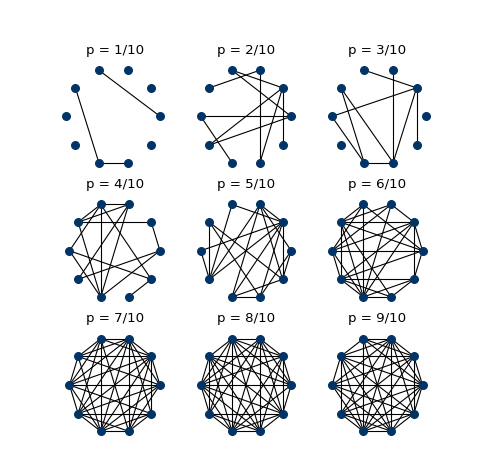
\includegraphics[scale=0.85]{Figures/ER-10.png}
	\caption{Erdös-Rényi random graphs with $n$ fixed and varying $p$}
	\label{fig:ErdosRenyi10}
\end{figure}

Figure \ref{fig:tiemposER} show the execution times varying $n$
\begin{figure}[h!]
	\centering
	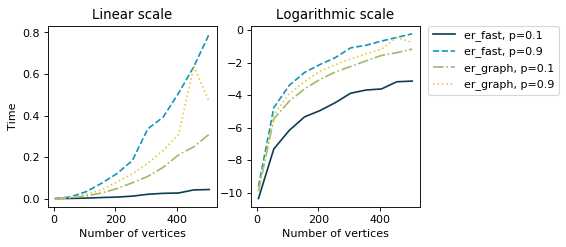
\includegraphics[scale=0.7]{Python/Figures/Time-execution-er-generation-algoriths.png}
	\caption{Execution times varying $n$. Both normal and logarithmic scale appear in the figure}
	\label{fig:tiemposER}
\end{figure}

\section{Rigid expansions algorithms}
A priory, the algorithm to determine a rigid expansion is supposed to be executed in a large amount of time. As the definition let us see, it depends on the size of $G$, and exponentially on the size of $A$; it must check among all the possible subsets of $A$, that's $2^{m}$ verifications, where $|A|=m$. Thus, it is important to do some optimization to the algorithms and evaluate when this have more impact in the expected execution time according to the parameters taken.

The following is the straightforward algorithm for rigid expansions.

\begin{cajita}
\textbf{Rigid Expansions Algorithm} \hfill \break

\begin{tabular}{ l l }
\texttt{Input:} &  \texttt{Random graph $G$ (dictionary),} \\
                &  \texttt{set of vertices $A$ (array).}\\
\texttt{Output:} & \texttt{Set of vertices obtained after expanding $A$ (array)} \\
\end{tabular}
\begin{enumerate}
\item Initialize N as empty (the set of new vertices)
\item For every $B$, subset of A:\hfill \break
\hphantom{12} If $\bigcap\limits_{b\in B} N(b) = v$ and $v\not\in A\cup N$: \hfill \break
\hphantom{1234} Add $v$ to $N$
\item If $N$ is not empty: \hfill \break
\hphantom{12} Replace $A$ by $A\cup N$ and return to step 1. \hfill \break
      Otherwise:\hfill \break
\hphantom{12} Return $A$
\end{enumerate}
\end{cajita}

To optimize memory in step two the iterations were indexed by \texttt{generators}. For time-execution optimizations, we implemented the following:

\begin{enumerate}
\item \textbf{Consideration of isolated vertices and leaves.} None of the isolated vertices in $G$ have any influence in rigid expansions, so they should not be consider. Also, whenever $A$ contains a leave is convenient to ignore them; the unique neighbor of a leave, which we will call \textit{petioles} should be automatically added in the first expansion an then it does not contribute in uniquely determine new vertices. This means that the input should be replace with:
$$A' = A - \{v: deg(v)\leq 1 \} \cup \{u: \exists x, N(x)=\{u\}\} $$
and add them again by the end of the expansions. This will be particularly helpful for small values of $p$.
\item \textbf{Relative size of $A$.} In Step 2, if $A$ is big enough is faster to check if a vertex outside of $A$ can be uniquely determinate by a subset of $A$. This can reduce dramatically the execution time when $p$ is small; it reduce the size of revisions by taking only the \textit{effective} part of $A$, this is convenient to do whenever
$$k\cdot log(2) > log(n-k) + (kp)\cdot log(2)$$
where $k$ is the size of $A$

\item \textbf{Restriction to effective subsets}. Calculations in Chapter 2 showed that some subsets are more likely to generate rigid expansions than others. This depend on the parameters of the space and the size of the subsets. If we restrict verifications to these effective subsets we can reduce the number of verifications.
\end{enumerate}

With these optimizations we obtain the following algorithm

\begin{cajita}
\textbf{Optimized Rigid Expansions Algorithm} \hfill \break

\begin{tabular}{ l l }
\texttt{Input:} &  \texttt{Random graph $G$ (dictionary),} \\
                &  \texttt{set of vertices $A$ (array),} \\
                &  \texttt{$n$(int) and $p$(float)} \\
\texttt{Output:} & \texttt{Set of vertices obtained after expanding $A$ (array)} \\
\end{tabular}
\begin{enumerate}
\item Replace $A$ by $A'$
\item Initialize $N$ as petioles of $A$ (the set of new vertices)
\item Calculate the range of effective subsets.\hfill \break
If $k\cdot log(2) > log(n-k) + (kp)\cdot log(2)$: \hfill \break
\hphantom{12} For every $v\in V-A$:\hfill \break
\hphantom{1234} Take $C = A\cap N(v)$ and for every $B$, effective subset of C:\hfill \break
\hphantom{123456} If $\bigcap\limits_{b\in B} N(b) = v$ and $v\not\in A\cup N$: \hfill \break
\hphantom{12341234} Add $v$ to $N$

Otherwise:\hfill \break
\hphantom{12} For every $B$, effective subset of A:\hfill \break
\hphantom{1234} If $\bigcap\limits_{b\in B} N(b) = v$ and $v\not\in A\cup N$: \hfill \break
\hphantom{123456} Add $v$ to $N$

\item If $N$ is not empty: \hfill \break
\hphantom{12} Replace $A$ by $A\cup N$, initialize $N$ as empty and return to step 3. \hfill \break
      Otherwise:\hfill \break
\hphantom{12} Return $A\cup\{v: deg(v)\leq 1 \}$
\end{enumerate}
\end{cajita}

\section{Time execution comparison}
We know that, given a $G\in\G(n,p)$ and a subset $A$ of $k$ vertices, the task of finding the first rigid expansion of $A$ in $G$ depends on $n,p,k$. To keep track of the execution time for the optimizations implemented, we measured the time for the rigid expansion varying the parameters. We took $k$ in some proportion of $n$, explicitly: $1/4$, $1/2$ and $3/4$, and for each collection of $n,p,k$ we measured the execution time for 30 different rigid expansions and afterwards we took a mean.

\begin{figure}[h!]
	\centering
	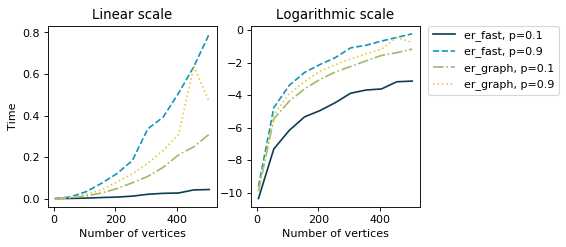
\includegraphics[scale=0.7]{Python/Figures/Time-execution-er-generation-algoriths.png}
	\caption{Execution times varying $n$. Both normal and logarithmic scale appear in the figure}
	\label{fig:tiemposER}
\end{figure}

Because of the nature of rigid expansions we expect to see an exponential increment of the time a rigid expansion takes when increasing $n$, also considering that we must execute the tests for a. Notice as well that several optimizations ahve more impact in sparse graphs 

\begin{figure}[h!]
	\centering
	\includegraphics[scale=0.7]{Python/Figures/Time-execution-rigi.png}
	\caption{Execution times varying $n$. Both normal and logarithmic scale appear in the figure}
	\label{fig:tiemposER}
\end{figure}




\section{Conclusions}

Probabilistic optimization and the understanding the combinatorial nature of rigid expansions allowed us to execute experiments for larger graphs that otherwise could not have been performed.

In general, the use of probability theory in computational has demonstrated to be powerful and efficient. Algorithms based in random sampling provide state-of-the-art techniques due to their great degree of flexibility and reliability. 

To name a few:
\begin{itemize}
\item The PageRank algorithm was the first method used by Google to order search results \cite[Page 99]{pageRank}. It outputs a probability distribution used to represent the likelihood that a person randomly clicking on links will arrive at any particular page.
\item In motion planning, the use of Rapidly-exploring random trees (RRTs) are one of the most successful algorithms \cite[Alcazar 15]{Alcazar15}. Problems in motion planning consist on finding a collision-free path that connects an initial configuration of geometric bodies to a final goal configuration. A RRT is a rooted tree that grows from a starting configuration by using random samples from the search space.
\end{itemize}

But it also works in the opposite direction, the use of computational tools can bring value for theoretical means. For theoretical means it has allowed, for example, to verify whether the established conditions in a probabilistic model are sharp enough (\cite[Aronshtam 13]{Meshulam13}).

Bottom line, the use of computational tools can be very helpful to understand a topic even in the most theoretical contexts.